\documentclass{article}
\usepackage{tikz}
\usetikzlibrary{arrows.meta}

\begin{document}

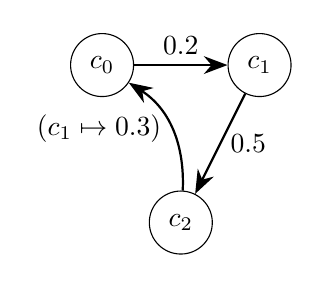
\begin{tikzpicture}[
    node distance=2cm,
    compartment/.style={circle, draw, minimum size=0.8cm},
    arrow/.style={-{Stealth[length=3mm]}, thick}
]

% Nodes
\node[compartment] (c0) at (0,0) {$c_0$};
\node[compartment] (c1) at (2,0) {$c_1$};
\node[compartment] (c2) at (1,-2) {$c_2$};

% Edges with labels
\draw[arrow] (c0) -- node[above] {$0.2$} (c1);
\draw[arrow] (c1) -- node[right] {$0.5$} (c2);
\draw[arrow] (c2) to[bend right=30] node[left] {$(c_1 \mapsto 0.3)$} (c0);

\end{tikzpicture}

\end{document}